\newpage
\chapter{Trade-Off Method}
\label{ch4-method}

%In this chapter the trade off between vehicle concepts will be extensively discussed. The objective is to select a combination of vehicle size and network type that best suits the demand in Los Angeles. Initially, the method, rationale and organization of this trade-off process will be elaborated upon in section \ref{sec:MRO}, after which the trade off criteria will be presented in section \ref{sec:Criteria}. Following this will be a selection of tools used for the criteria in section \ref{sec:Tools} and a sensitivity analysis in section \ref{sec:sensitivityanalysis}. 

In order to start the trade-off, the trade-off method has to be chosen. Four different methods are investigated and summarized in this chapter (\autoref{exp} to \autoref{graph}), this is followed by a comparison of these methods in \autoref{comp}. Also the method for the main trade-off during the Mid Term review is chosen in this section.

\section{Experience Based Trade-off}
\label{exp}
This method does not use any modelling or quantification of the different criteria and solutions, but is purely dependent onto the experience of experts. The estimates of multiple experts are compared and might be revised, when the deviations are too large. The advantage of this method that the trade-off can be performed with little data and without extensive measurements. If the expert already has the experience beforehand the method is fast, however if the experience still has to be gathered, this will be very time-consuming. A further disadvantage is that the trade-off cannot be replicated and some subjectivity might be present in the decision making \cite{tradeoff}.

\section{Traditional method}
A method to determine the weighting values of the criteria is by repeatedly comparing two criteria and determining which one is deemed to be more important. By doing this for each combination of criteria, a ranking of importance of the criteria can be created. This ranking can be converted to weighting factors, which then can be multiplied by the quantitative amount during the trade-off. The advantage of this technique is that the process can be performed by the whole team, thus creating more 'reliable' weighting factors. However, the ranking does not directly provide the weighting factors, so these have to be manually chosen. Also by this technique it can be clearly determined which criterion is considered most important by the team. Also, it can lead to discussions when two criteria are very evenly matched. Furthermore, the robustness of the system has to be analyzed by performing a sensitivity analysis on the weights. 

\section{Analytical Hierarchy Process}
A third technique that is analyzed is the Analytical Hierarchy Process (AHP), created by T.L. Saaty \cite{AHP}. This method is quite similar to the previous, but uses a slightly different way in comparing the criteria. Again, a pairwise comparison is performed for the criteria, but now also a value in the range of 1 to 9 is given, where 1 means equal importance and 9 means extremely more important. An example for such a ranking system is given in \autoref{AHP1}.

\begin{figure}[H]
    \centering
    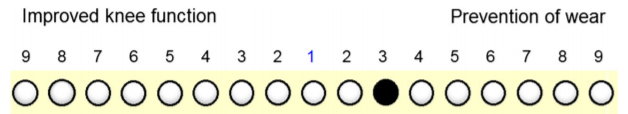
\includegraphics[width=0.75\linewidth]{Figures/AHP1.PNG}
    \captionsetup{justification=centering}
    \caption{Example of an AHP ranking of criteria \cite{AHPtut}}
    \label{AHP1}
\end{figure}

With $n$ criteria, a $n \times n$ matrix is created where the relative importance is shown. The rows are then multiplied and the $n^\text{th}$ root is taken, to normalize the values. In \autoref{AHP}, an example of a trade-off table using AHP is shown. It can be seen in the first row that time and work are considered respectively 3 and 6 times as important as the location. In the final column, the normalized priorities are placed, showing work as the main priority. These values can now be used as weighting factors, which are then multiplied by the quantitative values of each criterion. 

\begin{table}[H]
    \centering
    \captionsetup{justification=centering}
    \caption{Example of an AHP table to determine criterion weights \cite{AHP}} \vspace{-0.2cm}
    \label{AHP}
    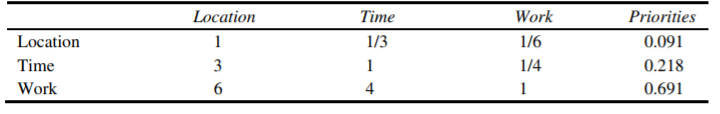
\includegraphics[width=0.75\linewidth]{Figures/AHP.PNG}
\end{table}

The advantage of AHP is that it is a repeatable technique, which is capable of comparing detailed and complex systems. However, the results should not be considered as exact as they seem. A sensitivity analysis should still be performed, to observe the differences in outcome when the relative scores are varied \cite{tradeoff}. 

\section{Graphical comparison method}
\label{graph}
Finally, also illustrative trade-off techniques exist. In these techniques a visual model is created, which shows the relations between the different criteria. This technique can provide great communicative possibilities, however the trade-off is simpler than a mathematical approach like AHP. Also the graphical method is mostly dependent on qualitative values and it is difficult to compare detailed concepts or systems \cite{tradeoff}.

\section{Comparison}
\label{comp}
When comparing the four different trade-off methods, two can clearly be excluded: The experience based trade-off and the graphical comparison method. The team has too little experience to choose a concept just based on its expertise and without really computing quantitative values or performing qualitative analyses. Furthermore, a graphical model for the concepts would not cover the complexity of these systems, so this would not aid in the decision making during the Mid-Term.

The two remaining methods both give a weighting factor to each criteria, that is then multiplied by the qualitative or qualitative value of that criteria. In terms of weighing the criteria there are also similarities, namely comparing the different criteria and determining which one would be more important. However, in the traditional method a ranking is made that is only dependent on which of the criteria is regarded to be more important, whereas in the AHP method scores are given dependent on the level of importance. Due to the large number of available research on the AHP method and the way the weighting factors are directly produced by the method, this will be the method that is used for this trade-off. 




